\documentclass{beamer}
\usepackage[spanish]{babel}
\usepackage[utf8]{inputenc}
\usepackage{graphicx}
\usetheme{Hannover}
\title{Clasificación de Información usando Redes Neuronales}
\subtitle{RNA}
\author{Alexis Peinado Rodriguez \and Ingrid Ipanaqué Casquina}

\institute[Universidad Nacional De Ingenieria]
{
  Ciencia de la Computación\\
  Universidad Nacional de Ingeniería
}

\date{Estadística y Probabilidades, \today}

\subject{Theoretical Computer Science}
\AtBeginSubsection[]
{
  \begin{frame}<beamer>{Clasificación de Información}
    \tableofcontents[currentsection,currentsubsection]
  \end{frame}
}
\begin{document}

\begin{frame}
  \titlepage
\end{frame}

\begin{frame}{Computer Science}
  \tableofcontents
\end{frame}

\section{Conceptos}

\subsection{Red Neuronal Artificial}

\begin{frame}{Red Neuronal Artificial}
\begin{block}{Principios}\pause
\begin{itemize}
\item {Aprendizaje Adaptativo\pause}
\item {Autoorganizativo\pause}
\item {Tolerancia a Fallos\pause}
\item {Operación en tiempo real\pause}
\item {Facil inserción en tecnología existente}
\end{itemize}
\end{block}
\end{frame}

\begin{frame}{Red Neuronal Artificial}
\begin{block}{Elementos}\pause
\begin{itemize}
\item {Elementos internos\pause}
\item {Capa o nivel\pause}
\item {Tipos de capas\pause}
\item {Conexion entre neuronas\pause}
\item {Dinámica}
\end{itemize}
\begin{figure}
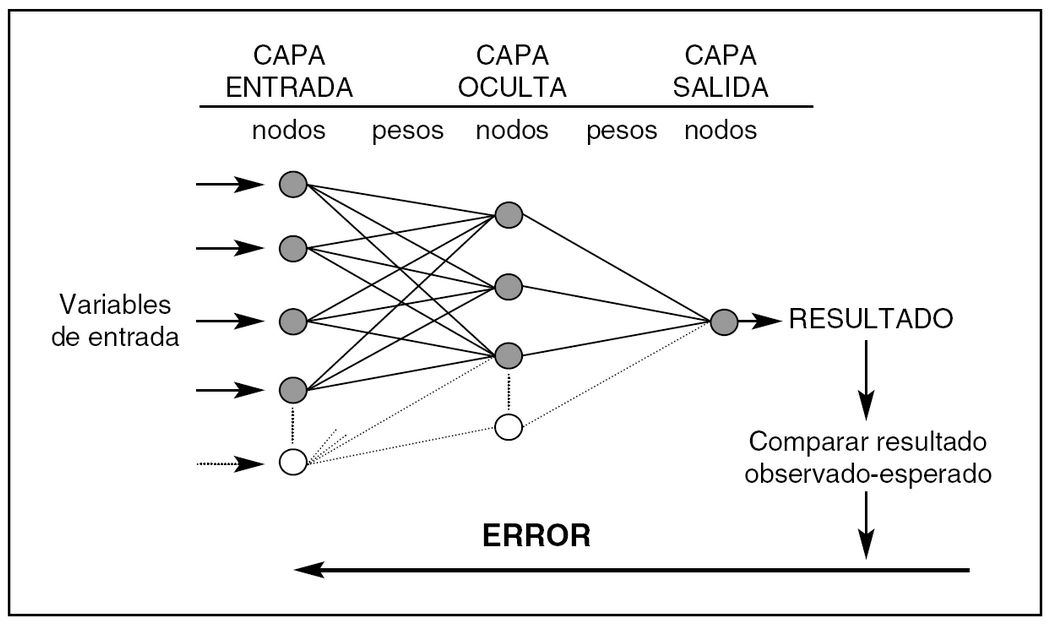
\includegraphics[scale=0.15]{elementos1.png}
\centering
\end{figure}
\end{block}
\end{frame}

\subsection{Aprendizaje Automático}
\begin{frame}{Aprendizaje Automático:}{Machine Learning}
\begin{itemize}
\item {Aprendizaje Supervisado\pause}
\begin{itemize}
\item {Aprendizaje por correcion de error\pause}
\item {Aprendizaje por refuerzo\pause}
\item {Aprendizaje estocástico\pause}
\end{itemize}
\item {Aprendizaje NO Supervisado\pause}
\begin{itemize}
\item {Aprendizaje hebbiano\pause}
\item {Aprendizaje competitivo}
\end{itemize}
\end{itemize}
\end{frame}

\section{Neurona y RNA}
\subsection{Neurona}
\begin{frame}{Neurona Y RNA}
\begin{block}{Neurona}
Células especializadas en la recepción de estímulos y conducción del impulso
nervioso.\pause
\begin{itemize}
\item {Dendritas\pause}
\item {Soma\pause}
\item {Axón\pause}
\item {Sinápsis\pause}
\item {Impulso Nervioso}
\end{itemize}
\begin{figure}
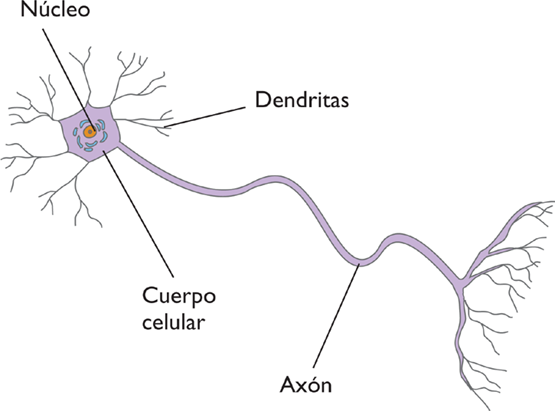
\includegraphics[scale=0.2]{neurona.png}
\centering
\end{figure}
\end{block}
\end{frame}

\subsection{RNA}
\begin{frame}{Neurona Y RNA}
\begin{block}{RNA}
Neurona el recibe una serie de entradas a través de interconexiones y emite una salida.\pause
\begin{itemize}
\item {Entradas\pause}
\item {Pesos Sinápticos\pause}
\item {Función de Propagación\pause}
\item {Funcion de Activación}
\end{itemize}
\begin{figure}
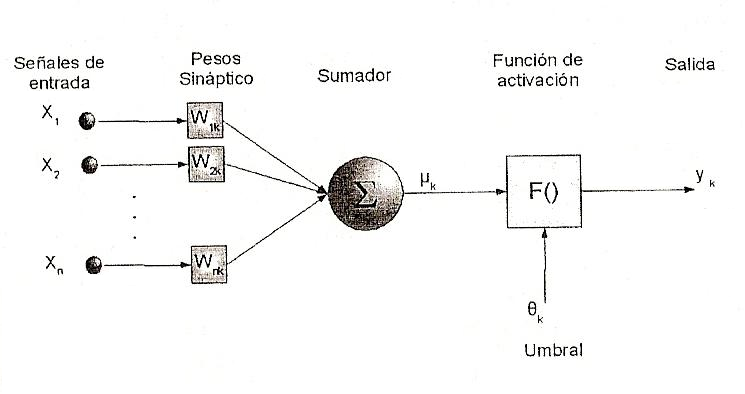
\includegraphics[scale=0.3]{rna.png}
\centering
\end{figure}
\end{block}
\end{frame}

\begin{frame}
\begin{center}
\begin{block}{Neurona Biológica y Neurona Artificial}
\begin{figure}
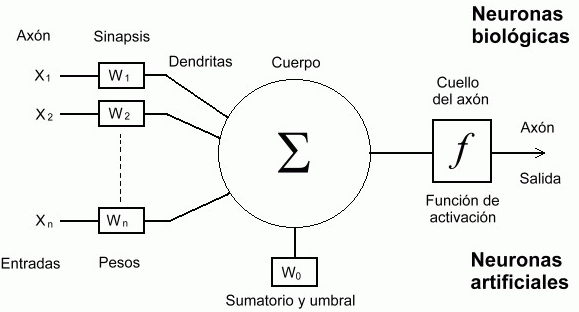
\includegraphics[scale=0.4]{Rna.png}
\centering
\end{figure}
\end{block}
\end{center}
\end{frame}

\section{Sistemas de Gestión de Información}
\subsection{Definición}
\begin{frame}
\begin{block}{Sistemas de Gestión de Información}
Un profesional infiere una estructura a partir de información documental no estructurada, el cual implementada en una aplicación informática permite con posterioridad recuperar información.
\begin{figure}
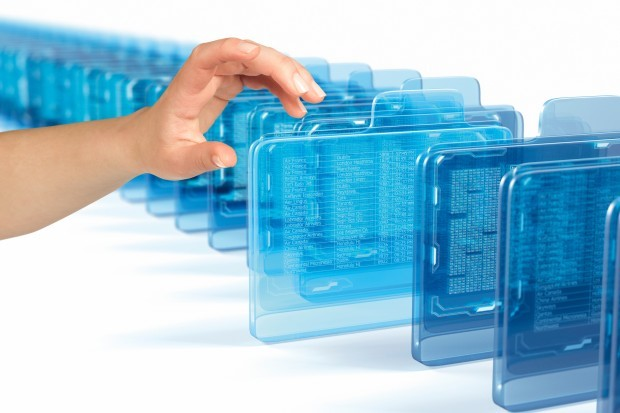
\includegraphics[scale=0.3]{gestion.jpg}
\centering
\end{figure}
\end{block}
\end{frame}

\subsection{Método de las Tablas Relacionales}
\begin{frame}
\begin{block}{Modelo Relacional}
Se utiliza para el modelado y la gestión de bases de datos, en este modelo todos los datos son almacenados en relaciones, pensando en cada relación como si fuese una tabla compuesta por registros y columnas.
\begin{figure}
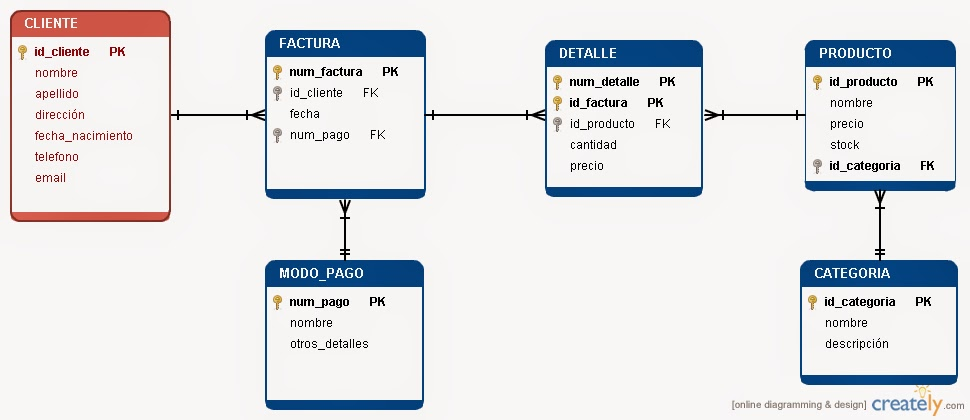
\includegraphics[scale=0.2]{ModeloRelacional.jpg}
\centering
\end{figure}
\end{block}
\end{frame}

\section{Implementación}
\subsection{Lenguaje R}
\begin{frame}{Lenguaje R}
\begin{block}{Características}
\begin{itemize}
\item Es un lenguaje de programación el cual permite que lo usuarios creen sus propias funciones.
\item Posee manipulación de objetos en R y además su \textbf{orientación a objetos.}
\item La facil extensión de R debido a su política de \textbf{lexical scoping}
\item La integración y la sencilla manipulación de base de datos.
\item Su capacidad gráfica, permite generar gráficos de alta calidad.\\
\end{itemize}
\end{block}
\end{frame}

\begin{frame}{Paquete de R}
\begin{block}{NeuralNet}
dwdwdw
\end{block}
\end{frame}


\begin{frame}{Paquetes de R}
\begin{block}{Kohonen}
El paquete kohonen tiene como objetivo proporcionar funciones fáciles de usar para los mapas de auto-organización, con especial énfasis en la visualización.
\end{block}
\end{frame}

\subsection{Aprendizaje Supervisado}
\begin{frame}
\begin{block}{Leyendo Tabla OR}
\begin{figure}
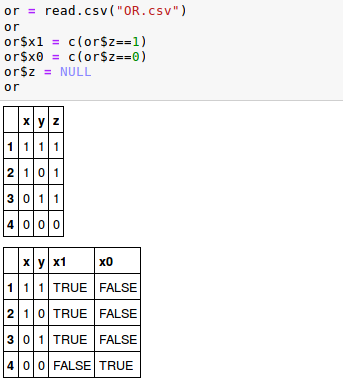
\includegraphics[scale=0.4]{reador.png}
\centering
\end{figure}
\end{block}
\end{frame}

\begin{frame}
\begin{block}{Entrenando RNA para puerta lógica OR}
\begin{figure}
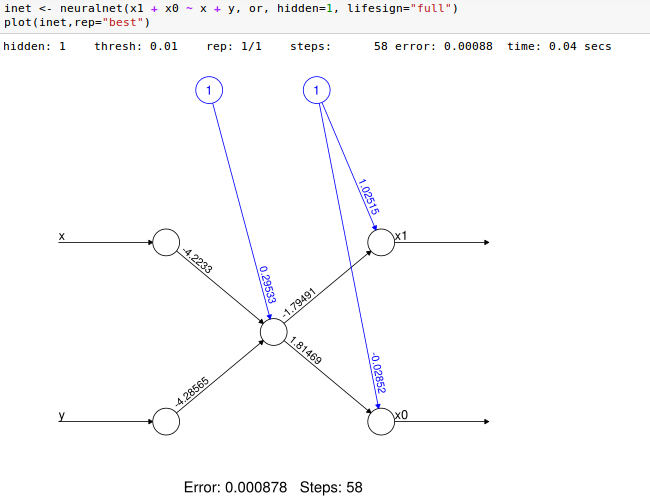
\includegraphics[scale=0.4]{neuralnetor.png}
\centering
\end{figure}
\end{block}
\end{frame}


\begin{frame}
\begin{block}{Leyendo Tabla AND}
\begin{figure}
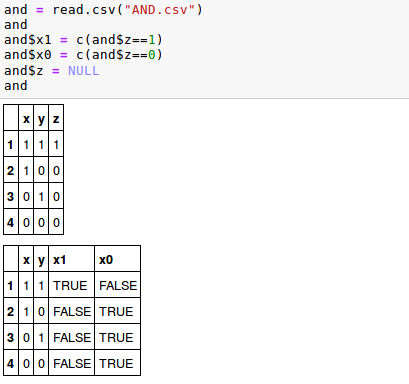
\includegraphics[scale=0.4]{readand.png}
\centering
\end{figure}
\end{block}
\end{frame}

\begin{frame}
\begin{block}{Entrenando RNA para puerta lógica AND}
\begin{figure}
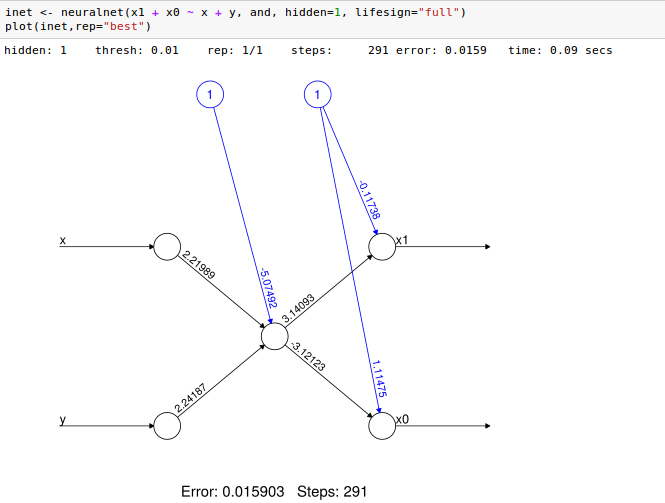
\includegraphics[scale=0.4]{neuralnetand.png}
\centering
\end{figure}
\end{block}
\end{frame}

\begin{frame}
\begin{block}{Leyendo Tabla XOR}
\begin{figure}
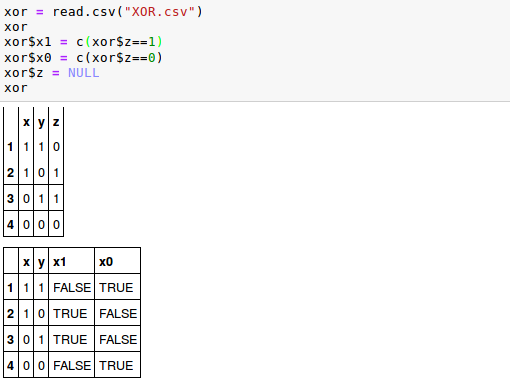
\includegraphics[scale=0.4]{readxor.png}
\centering
\end{figure}
\end{block}
\end{frame}

\begin{frame}
\begin{block}{Entrenando RNA para puerta lógica XOR}
\begin{figure}
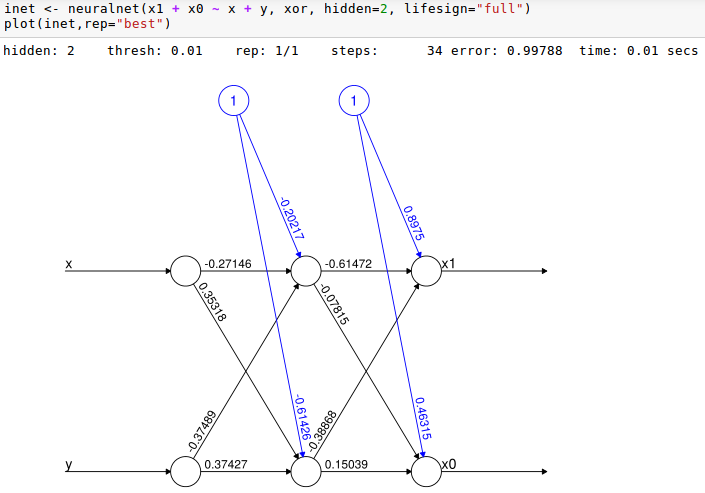
\includegraphics[scale=0.4]{neuralnetxor.png}
\centering
\end{figure}
\end{block}
\end{frame}

\begin{frame}{Base de Datos Iris}
\begin{block}{Entrenando Red}
\begin{figure}
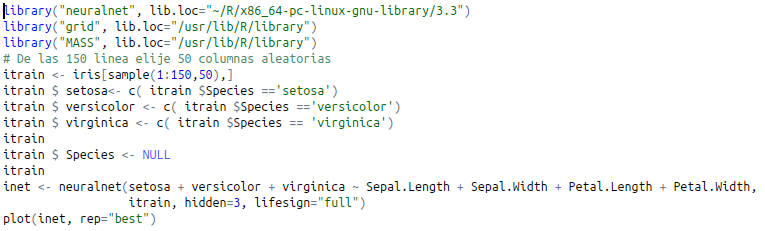
\includegraphics[scale=0.4]{entrenando.png}
\centering
\end{figure}
\end{block}
\end{frame}

\begin{frame}{Base de Datos Iris}
\begin{block}{Entrenando Red}
\begin{figure}
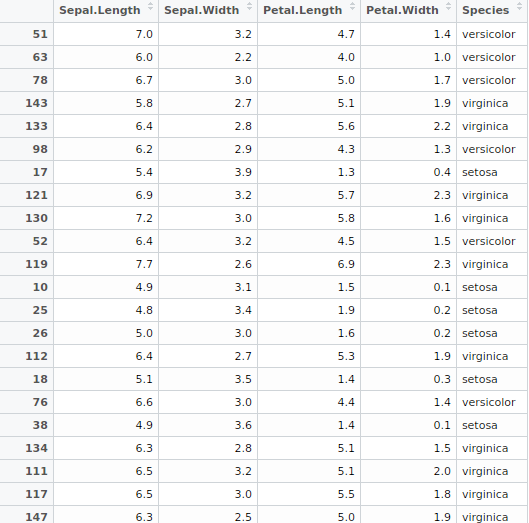
\includegraphics[scale=0.3]{tablairis.png}
\centering
\end{figure}
\end{block}
\end{frame}

\begin{frame}{Base de Datos Iris}
\begin{block}{Entrenando Red}
\begin{figure}
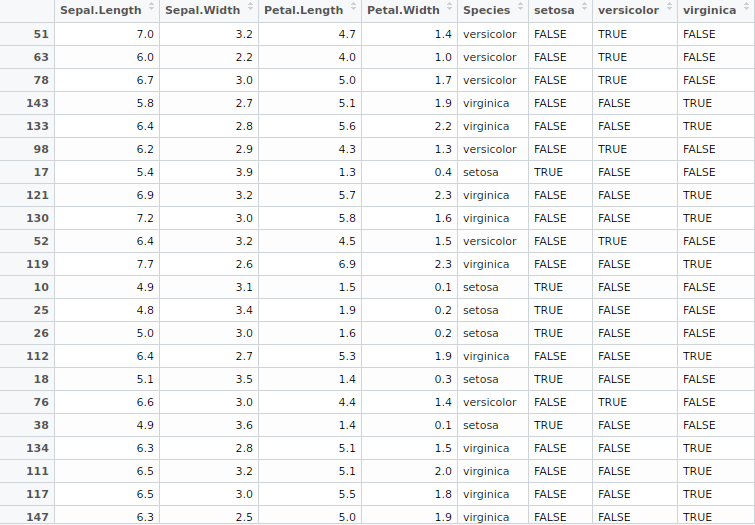
\includegraphics[scale=0.3]{irisespecie.png}
\centering
\end{figure}
\end{block}
\end{frame}

\begin{frame}{Base de Datos Iris}
\begin{block}{Entrenando Red}
\begin{figure}
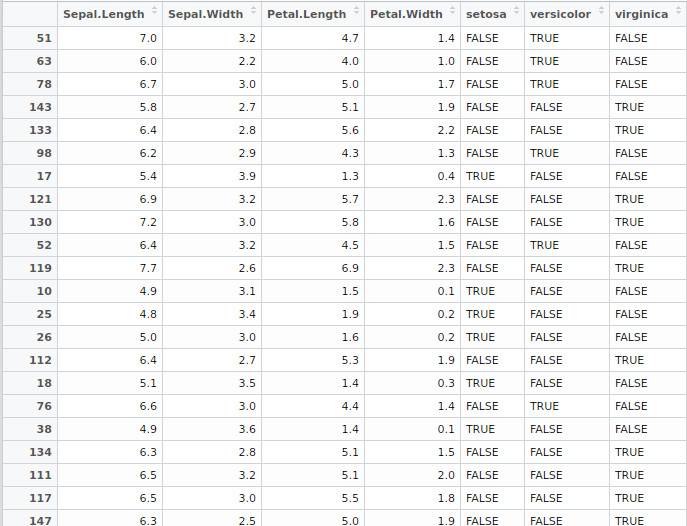
\includegraphics[scale=0.3]{irisfalsetrue.png}
\centering
\end{figure}
\end{block}
\end{frame}

\begin{frame}{Base de Datos Iris}
\begin{block}{Entrenando Red}
\begin{figure}
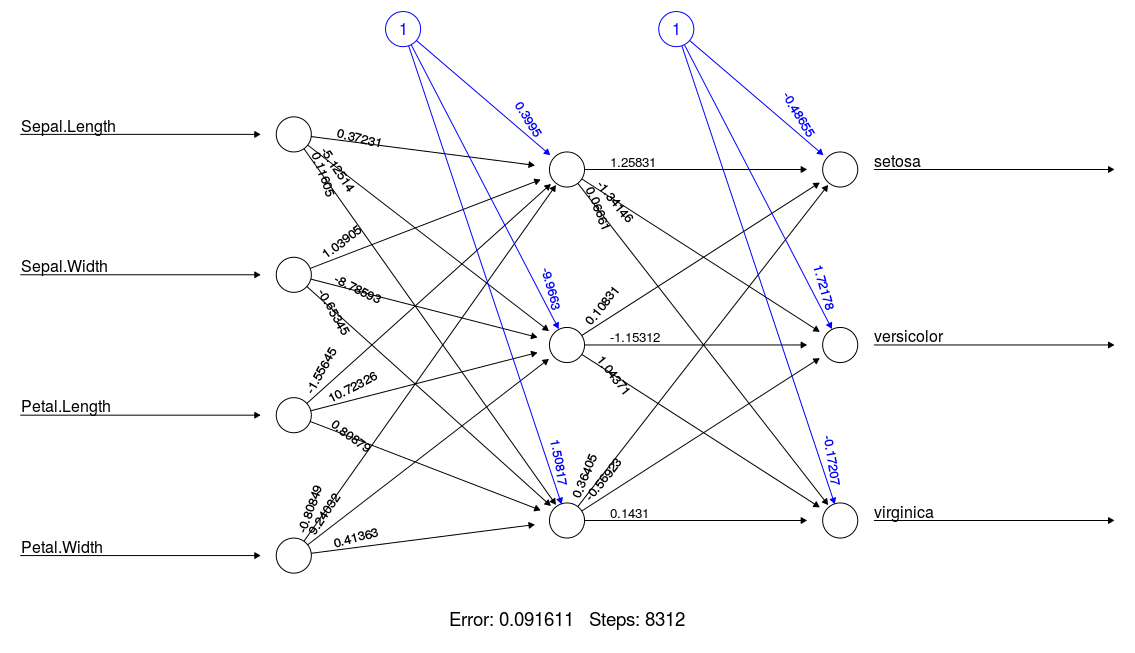
\includegraphics[scale=0.25]{entrenadairis.png}
\centering
\end{figure}
\end{block}
\end{frame}

\begin{frame}{Base de Datos Iris}
\begin{block}{Verificando Red}
\begin{figure}
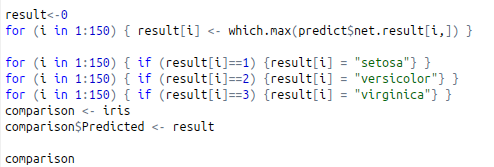
\includegraphics[scale=0.4]{comparando.png}
\centering
\end{figure}
\end{block}
\end{frame}

\begin{frame}{Base de Datos Iris}
\begin{block}{Verificando Red}
\begin{figure}
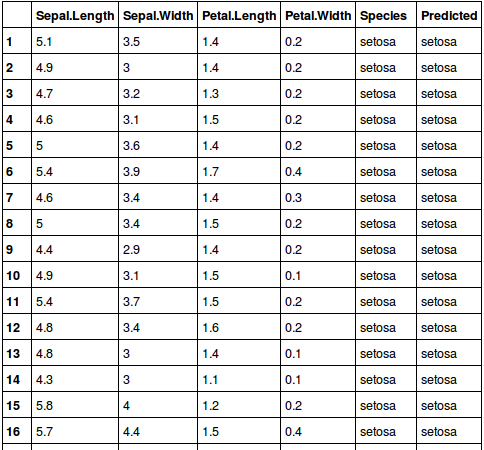
\includegraphics[scale=0.4]{comparacion.png}
\centering
\end{figure}
\end{block}
\end{frame}

\subsection{Aprendizaje NO Supervisado}

\begin{frame}{Base de Datos Iris}
\begin{block}{Entrenando Red}
\begin{figure}
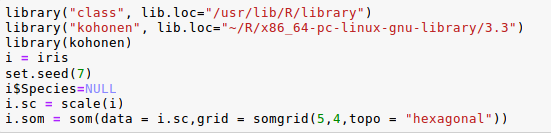
\includegraphics[scale=0.4]{mallairis.png}
\centering
\end{figure}
\end{block}
\end{frame}

\begin{frame}{Base de Datos Iris}
\begin{block}{type=codes}
\begin{figure}
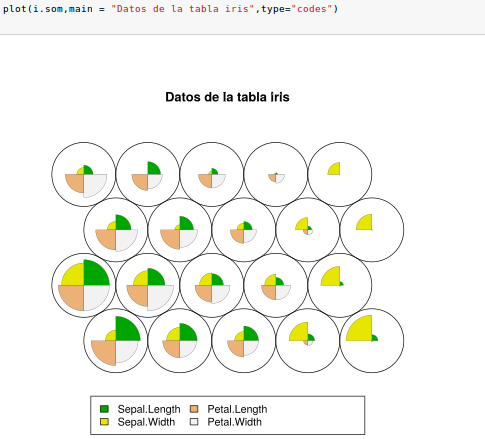
\includegraphics[scale=0.4]{codes.png}
\centering
\end{figure}
\end{block}
\end{frame}

\begin{frame}{Base de Datos Iris}
\begin{block}{type=changes}
\begin{figure}
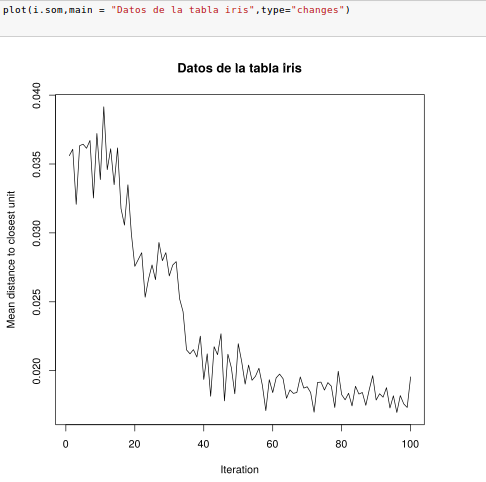
\includegraphics[scale=0.4]{changes.png}
\centering
\end{figure}
\end{block}
\end{frame}

\begin{frame}{Base de Datos Iris}
\begin{block}{type=counts}
\begin{figure}
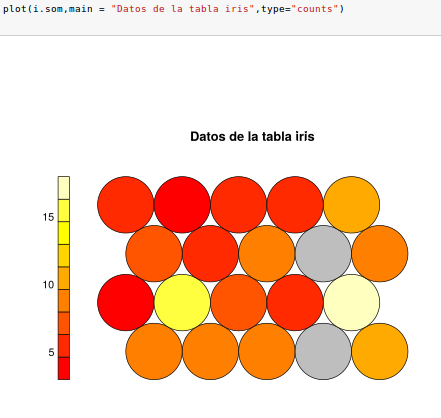
\includegraphics[scale=0.4]{counts.png}
\centering
\end{figure}
\end{block}
\end{frame}

\begin{frame}{Base de Datos Iris}
\begin{block}{type=neighbours}
\begin{figure}
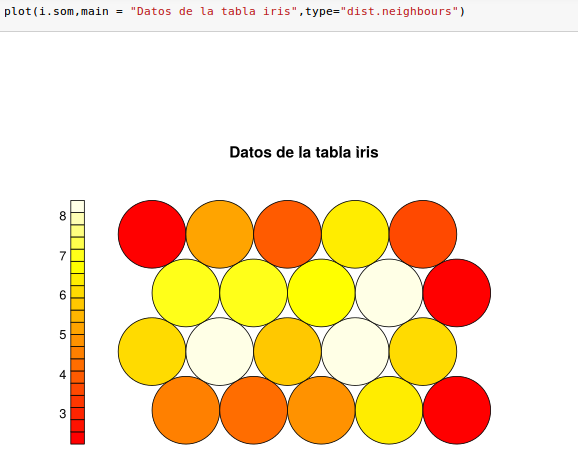
\includegraphics[scale=0.4]{neighbours.png}
\centering
\end{figure}
\end{block}
\end{frame}

\appendix
\section<presentation>*{\appendixname}
\subsection<presentation>*{Bibliografía}

\begin{frame}[allowframebreaks]
\frametitle<presentation>{Bibliografía}
    
\begin{thebibliography}{10}  
\beamertemplatebookbibitems
\bibitem{Francisco Gutierrez Martin}
A.~Author.
\newblock {\em Redes Neuronales Artificiales}.
\newblock Web: thales.cica.es, 2000.
 
\beamertemplatearticlebibitems

\bibitem{Research}
A.~Autor.
\newblock Aplicación de redes neuronales aritificiales a la recuperacion de información
\newblock {\em Felix de Moya Anegón, Victor Herrero Solana, Vicente Guerrero Bote}, 2000.

\beamertemplatearticlebibitems
\bibitem{Research2}
A.~Author.
\newblock Aplicaciones de redes neuronales aritificiales en documentación.
\newblock {\em Natividad Noverges, Vicente Sacristán, Pepa Ortí, Lourdes Margaix}, 2000-2001.

\end{thebibliography}
\end{frame}

\end{document}